% !TEX root = main.tex
%\myparagraph{Key points}
%\begin{enumerate}[1.]
%%	\item	Session $\pi$ calculus with process passing. DONE
%%	\item	Identify session $\pi$ and process passing subcalculi and their polyadic variants. DONE
%%	\item	Bisimulation theory for higher-order session semantics. DONE
%%	\item	New triggered bisimulation, related to J\&R's. DONE
%%	\item   Elementary values key to characterizations of behavioral equivalence. DONE
%	\item	Types provide techniques to prove completeness without matching. \jp{TBD}
%	\item	We are interested in encodings with properties a la Gorla. 
%                We extended them to typed setting. \jp{TBD}
%%	\item	Encode name-passing to pure process abstraction calculus, with name abstractions. DONE
%%	\item	Type of the recursion encoding uses non tail recursive type $\trec{t}{\btinp{t} \tinact}$. DONE
%%	\item	Encode higher-order semantics to first order semantics. DONE
%%	\item	Negative result. Cannot encode shared names using only shared names.
%%	\item   Extensions with higher-order abstractions and polyadicity also explored. DONE
%\end{enumerate}

%\smallskip 
%
%\myparagraph{Important things to explain}
%Explain our \HO is very small without containg name passing 
%\[ 
%\abs{x}.P \quad \appl{x}{u}
%\]

%Explain we input only characteristic processes.  
%
%\[
%\lambda x.\mapchar{S}{x}
%\]

%\subsection{Higher-Order Session Calculi}
\noi 
By combining features from the $\lambda$-calculus and the $\pi$-calculus, 
in \emph{higher-order process calculi} exchanged values may contain  processes. 
In this paper, we consider higher-order calculi with \emph{session primitives},
thus enabling the specification of sequences of reciprocal exchanges (protocols)
which can be verified via type-checking using \emph{session types}~\cite{honda.vasconcelos.kubo:language-primitives}.
These higher-order process languages allow us to specify   
session protocols in which higher-order values 
(mobile code) can be exchanged; governed by session types, 
such protocols cleanly distinguish between 
linear and unrestricted behaviors in 
%directed %point-to-point 
communications.

The study of higher-order concurrency has received significant attention, 
from typed and untyped perspectives.
%in particular via  comparisons with the first-order mobility of the $\pi$-calculus~\cite{MilnerR:calmp1}. 
Although models of session-typed 
communications with features of higher-order concurrency exist~\cite{tlca07,DBLP:journals/jfp/GayV10},
certain aspects of their theory 
remain little understood. Here we address
 \emph{tractable behavioral equivalences} and \emph{relative expressiveness}:
%for higher-order session calculi. 
these two issues 
have been throughly studied
%are well-understood 
for higher-order languages without sessions,
but not for higher-order process calculi with sessions.
This is unfortunate, given the wide applicability of session-based concurrency; indeed,
session types are expressive enough to describe complex 
communication structures found in practical protocols,  expressible, e.g., via recursive session types.
Clarifying the status of typed equivalences and relative expressiveness for session languages
may play a vital role in justifying non-trivial protocol optimizations and in transferring key reasoning techniques between session calculi.

The main higher-order language in our work, denoted \HOp,
extends the higher-order $\pi$-calculus~\cite{SangiorgiD:expmpa} with session primitives:
it contains constructs for 
%session establishment
synchronization on shared names, 
recursion, 
name abstractions/applications (i.e., functions from name identifiers to processes, call-by-value style),
and session communication (value passing and
labeled choice using linear names). 
Two significant subcalculi of \HOp restrict to higher- and first-order mobility:
while the \HO calculus is \HOp without recursion and name passing,
the \sessp calculus is \HOp without abstractions and applications.
Thus, 
while $\sessp$ is in essence the calculus in~\cite{honda.vasconcelos.kubo:language-primitives}, 
\HO  is  a core calculus for higher-order session concurrency.

In the first part of the paper, we address tractable behavioral equivalences
for \HOp.
A well-studied behavioral equivalence in the higher-order setting 
is \emph{context bisimilarity}~\cite{San96H},
a labelled characterization of barbed congruence, 
which offers an appropriate discriminative power at the price of heavy universal quantifications in output clauses.
Obtaining alternative characterizations that alleviate this burden
is then a recurring and important issue 
in the study of higher-order languages.
Our approach to this problem 
exploits the protocol specifications given by session types to  limit 
the behavior of higher-order session processes. 
Exploiting elementary processes inhabiting session types, 
this limitation is formally enforced by 
a refined (typed) labelled transition system (LTS)
that narrows down the spectrum of allowed process behaviors, 
thus naturally enabling tractable reasoning techniques. 
Two tractable characterizations of bisimilarity, 
targeted to higher- and first-order session processes,
are shown to coincide with contextual bisimilarity.

We then move on to 
%in the second part of the paper we 
assess the expressivity 
 of \HOp, \HO, and \sessp as delineated by typing. 
We establish strong correspondences between 
these languages via fully abstract encodings. 
Here again the usage information given by session types is essential to define encodings
and to state their semantic correspondences.
 Building upon established notions for (untyped) processes~(e.g.,~\cite{DBLP:journals/iandc/Gorla10}), 
 we
define a notion of \emph{precise encoding} that 
requires the translation of both process and types, and 
focuses on process mappings that preserve (session) typing. 
Thus, our encodings only relate source and target 
processes 
with  
proper communication structures (given by session types).
A further result shows that 
shared names
%as required in the session establishment phase,
 strictly add expressive power 
to session calculi. 
Fig.~\ref{fig:express} summarizes %our expressivity 
these
results.

\begin{figure}[t]
%ADD~FIGURE!
	\begin{center}
		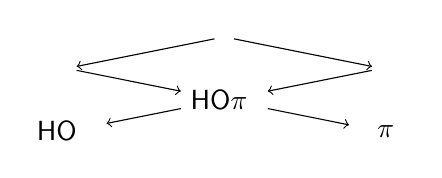
\begin{tikzpicture}
			\node	(PHOpp)	at	(0, 0.8)		{\PHOpp};
			\node	(HOpp)	at	(-2, 0.4)	{\HOpp};
			\node	(PHOp)	at	(2, 0.4)	{\PHOp};
			\node	(HOp)	at	(0, 0)		{$\mathsf{HO}{\pi}^{~}$};
			\node	(HO)	at	(-2, -0.4)	{$\mathsf{HO}{~}^{~}$};
			\node	(sessp)	at	(2, -0.4)	{$~~\pi^{~}$};

			\draw[->]	(PHOpp) -- (HOpp);	%(0, 1.25) -- (-2, 1);
			\draw[->]	(PHOpp) -- (PHOp);	%(0, 1.25) -- (2, 1);

			\draw[->]	(HOpp) -- (HOp);	%(2, 0.5) -- (0, 0.25);
			\draw[->]	(PHOp) -- (HOp);	%(-2, 0.5) -- (0, 0.25);

			\draw[->]	(HOp) -- (HO);		%(0, -0.25) -- (-2, -0.5);
			\draw[->]	(HOp) -- (sessp);	%(0, -0.25) -- (2, -0.5);


			% Polyadic HO and Polyadic pi
	%		\node	at	(-3, 0)		{\PHO};
	%		\node	at	(3, 0)		{\Psessp};

	%		\draw[->]	(0, 1.5) -- (-3, 0.25);
	%		\draw[->]	(0, 1.5) -- (3, 0.25);

	%		\draw[->]	(3, -0.25) -- (2, -0.5);
	%		\draw[->]	(-3, -0.25) -- (-2, -0.5);




		\end{tikzpicture}
	\end{center}
\caption{Summary of Expressiveness Results. \label{fig:express}}
\Hline
\end{figure}

\smallskip

\myparagraph{Outline.}
Next  we overview our results and approach.
\noi \S\,\ref{sec:calculus} presents the calculi; 
\S\,\ref{sec:types} presents types.
The tractable bisimulations are in \S\,\ref{sec:behavioural}.
The notion of encoding is in \S\,\ref{s:expr} and
\S\,\ref{sec:positive} %and \S\,\ref{sec:negative}
presents expressiveness results.
%present positive and negative encodability results, resp;
In \S\,\ref{sec:extension} we discuss extensions; 
\S\,\ref{sec:relwork} concludes with related works.
An appendix summarises the typing system. 
The paper is self-contained. 
{\bf\em Omitted definitions, additional related work, and  proofs 
%can be found
are 
in~\cite{KouzapasPY15}.} 

\section{Overview}
\label{sec:overview}
\noi
%In  
%\S\,\ref{subsec:intro:expr}
%and
%\S\,\ref{subsec:intro:bisimulation}
We motivate further our contributions and 
give details of the technical challenges involved. 
Some  notation, formally introduced shortly, is useful here:
$\bout{u}{V} P$
and
$\binp{u}{x} P$ denote input- and output-prefixed processes.
Values $V, W$ can be either a name $u$ or an (name) abstraction $\abs{x}Q$.
Processes $P \Par Q$ and $\inact$ denote the parallel composition and inactive processes, respectively.
Given a (linear) session name $s$, we write $\dual{s}$ for its \emph{dual}; 
they are the two \emph{endpoints} of the same session: the restriction operation  
$\news{s}P$ simultaneously covers $s$ and $\dual{s}$ in~$P$. 
The restriction for shared name $a$ in $P$ is denoted $\news{a}P$.
We write $S$ to range over session types;
this way, e.g., session type $\btout{U} S'$ (resp. $\btinp{U} S'$) is
decrees that the output (resp. input) of a value of type $U$
must precede a protocol with type $S'$. 
The  terminated session is typed with $\tinact$.
%Given  type $U$, 
We write $\lhot{U}$ (resp. $\shot{U}$) for the 
linear (resp. unrestricted) functional type.

\subsection{Relative Expressiveness Results}
\label{subsec:intro:expr}
\myparagraph{Encoding Name Passing and Recursion into \HO.}
Our first encodability result highlights the expressiveness of 
the core higher-order calculus \HO, which lacks name passing and recursion. 
We encode \HOp into \HO, which entails also an encoding of \sessp into \HO.
The challenges in this encoding of concern exactly name passing and recursion.
To encode name output, we ``pack''
the name to be passed around into a suitable abstraction; 
upon reception, the receiver must ``unpack'' this object following a precise protocol.
The encoding formally is defined in Def.~\ref{d:enc:hopitoho}; we illustrate the encoding strategy below.
The encoding of name passing is:
\[
\begin{array}{rcll}
  \map{\bout{u}{w} P}	&=&	\bout{u}{ \abs{z}{\,\binp{z}{x} (\appl{x}{w})} } \map{P} \\
  \map{\binp{u}{x} Q}	&=&	\binp{u}{y} \newsp{s}{\appl{y}{s} \Par \bout{\dual{s}}{\abs{x}{\map{Q}}} \inact}
\end{array}
\]
and so we need 
exactly two (deterministic) reductions 
to unpack  name $w$.
The encoding of a recursive process $\recp{X}{P}$  is delicate, for it 
 must preserve the linearity of session endpoints. To this end, we
%\begin{enumerate}[i)]
%\item 
encode the recursion body $P$ as a (polyadic) name abstraction
in which free session names are converted into name variables.
This higher-order value is embedded in a sort of input-guarded 
``duplicator'' process; the encoding of process variable $X$ is then meant to 
invoke the duplicator in a by-need fashion to simulate recursion unfolding. 

%\item The recursion body $P$ is encoded in such a way that
%the  in $\map{P}$ (linear names) ; the obtained process
%is then used as the body of a  on those variables.
%\item Using a private session, the abstraction obtained in (i) is communicated to a
%process which instantiates the initial free session names in $P$, 
%in coordination with the encoding of the recursion variable $X$ (using a private session).
%\end{enumerate}
%The second step is also challenging:
%in essence, one should establish a private session with the encoding of the recursion  
%body in order to spawn copies of $\map{P}$ with appropriate free session names.
The use of polyadicity is crucial to the encoding; we shall get back to this point below.
It is worth noticing that the typing of the encoding requires 
a non tail recursive type of the form $\trec{t}{\btinp{\lhot{(S,\vart{t}}} \tinact}$
(see Def.~\ref{d:enc:hopitoho} for the precise formulation).

\smallskip 

\myparagraph{Other Encodings.}
We also give %the reverse of the previous encoding, namely 
an encoding of \HOp into \sessp. We rely on the well-known representability result of Sangiorgi~\cite{SangiorgiD:expmpa}. 
Since communicated processes may contain session names, in order to respect linearity and session protocols
the encoding enforces a distinction, depending on whether this kind of names is present in the communication object. If session names are present then a linear server trigger is deployed; otherwise, the replicated server  in~\cite{SangiorgiD:expmpa} can be used. 

As mentioned above, \HOp and \HO feature \emph{first-order} abstractions: 
only names can be used as arguments to abstractions.
Hence, given a (shared/linear) name $u$, in \HOp
we have the reduction $(\abs{x}{P}) \, u   \red  P \subst{u}{x}$.
We also consider \HOpp, an extension of \HOp with \emph{higher-order} abstractions.
 Thus, in \HOpp also an arbitrary value $V$ (possibly a process) can be an argument of an abstraction, 
 and one could have the reduction
 $(\abs{x}{P}) \, V   \red  P \subst{V}{x}$.
 We give an encoding of \HOpp into \HO: it  naturally extends that of \HOp into \HO;
see~\S\,\ref{subsec:hop}.

A well-known feature in process calculi is \emph{polyadicity}, i.e.,  
passing around tuples of values in communications. 
We consider the polyadic extension of \HOp, denoted \pHOp.
In \pHOp we have polyadicity in session communications and abstractions; 
polyadicity of shared names is ruled out by typing. 
This is enough for most purposes, including our encoding from \HOp into \HO.
In a session-typed setting, encoding polyadicity is straightforward, thanks to 
%polyadic arguments can be sent one by one, relying on 
the private character of 
(linear) session names --- see \S\,\ref{subsec:pho} for details.
%\[
%\begin{array}{rl}
%		\map{\binp{u}{x_1, \cdots, x_m} P}
%		 =  & \!\!\!\!
%		\binp{u}{x_1} \cdots ;  \binp{u}{x_m} \map{P}
%		\\
%%		\map{\bout{u}{u_1, \cdots, u_m} P}
%%		 =  & \!\!\!\!
%%		\bout{u}{u_1} \cdots ;  \bout{u}{u_m} \map{P}
%%		\\
%		\map{\bbout{u}{\abs{(x_1, \cdots, x_m)} Q} P}
%		= & \!\!\!\!
%		\bbout{u}{\abs{z}\binp{z}{x_1}\cdots ; \binp{z}{x_m} \map{Q}} \map{P}
%		\\ 
%		\map{\appl{x}{(u_1, \cdots, u_m)}}
%		= & \!\!\!\!
%		\newsp{s}{\appl{x}{s} \Par \bout{\dual{s}}{u_1} \cdots ; \bout{\dual{s}}{u_m} \inact} 
%	\end{array}
%\]
%Notice that encoding of polyadic abstraction/application requires an extra step, 
%in which a monadic abstraction is sent.

\smallskip

\myparagraph{A Non Encodability Result.}
We also show that shared names strictly add expressiveness to session calculi: that is,
there are (non deterministic) behaviors expressible with shared names not expressible using linear names only.
Although somewhat expected we do not know of a formal proof.
We propose such a formal proof, which relies crucially on the behavioral theory that we have introduced here
and on its determinacy properties. %\jp{EXPAND}.


\subsection{Tractable Bisimilarities for Session-Typed Processes}
\label{subsec:intro:bisimulation}
\noi 
\myparagraph{Overcoming Issues of Context Bisimilarity.}
%The characterisation of contextual congruence given by 
Context bisimilarity ($\wbc$, Def.~\ref{def:wbc}) is a too demanding relation on processes. 
%In the following we motivate our
%proposal for alternative, more tractable characterisations.  
%For the sake of clarity, and to emphasise the novelties of our approach, 
%we often omit type information. 
%Formal definitions including types are in \S\,\ref{sec:behavioural}.
To see the issue, we show 
the following clause for output.
Suppose $P \,\Re\, Q$, for some context bisimulation $\Re$. Then:

\smallskip 

\begin{enumerate}[$(\star)$]
\item Whenever 
$P \by{\news{\tilde{m_1}} \bactout{n}{V}} P'$
there exist
$Q'$ and $W$
such that 
$Q \by{\news{\tilde{m_2}} \bactout{n}{W}} Q'$
and, for all $R$ with $\fv{R}=x$, 
$\newsp{\tilde{m_1}}{P' \Par R\subst{V}{x}} \,\Re\, \newsp{\tilde{m_2}}{Q' \Par R\subst{W}{x}}$.
\end{enumerate}
\smallskip 
\noi 
Above, 
$\news{\tilde{m_1}} \bactout{n}{V}$ is the output label of 
value $V$ with extrusion of names in $\tilde{m_1}$.
To reduce the burden induced by 
universal quantification, we introduce \emph{higher-order}  and 
\emph{characteristic}  
bisimulations, two tractable equivalences denoted  $\hwb$ and $\fwb$, respectively.
As we work with an \emph{early} labelled transition system (LTS), 
we shall also aim at limiting the input actions,  
so to define a
bisimulation relation for the output clause without observing
infinitely many actions on the same input prefix. 
To this end, we take the following two steps: 
%
\begin{enumerate}[(a)]
	\item We replace $(\star)$ with a clause involving a more tractable process closure.
	\item We refine the transition rule for input in the LTS.
\end{enumerate}
%
\smallskip

\myparagraph{Trigger Processes with Session Communication.}
Concerning~(a), we exploit session types. 
We 
first 
observe that closure $R\subst{V}{x}$ 
in $(\star)$
is contextually bisimilar to the process
\begin{equation}\label{equ:1}
P = \newsp{s}{\appl{(\abs{z}{\binp{z}{x}{R}})}{s} \Par \bout{\dual{s}}{V} \inact}
\end{equation}
\noi 
%where $\binp{z}{x}{R}$ is an input and $\bout{\dual{s}}{V} \inact$
%is an output 
%on the endpoint $\dual{s}$ (the dual of $s$).
In fact,
we have $P \wbc R\subst{V}{x}$, 
since 
application and reduction of dual endpoints 
%($s$ and $\dual{s}$) 
are deterministic.  
Now consider process $T_{V}$ below, where $t$ is a fresh name:
\begin{equation}\label{equ:0}
T_{V} = \hotrigger{t}{V}
\end{equation}
%We call $\abs{z}{\binp{z}{x} R}$ a {\bf\em trigger value}. 
If $T_{V}$ inputs $\abs{z}{\binp{z}{x} R}$
we can simulate the closure of $P$:
\begin{equation}\label{equ:2}
%\hotrigger{t}{V_1} 
T_{V}
\by{\bactinp{t}{\abs{z}{\binp{z}{x} R}}} P 
\wbc 
R\subst{V}{x}
\end{equation}
Processes such as $T_{V}$ 
offer a value at a fresh name; we will use this class of 
{\bf\em trigger processes} to define a
 refined bisimilarity without the demanding 
output clause $(\star)$. Given a fresh name $t$, 
we write $\htrigger{t}{V}$ to 
stand for a trigger process $T_{V}$ for value $V$.
We note that 
in contrast to previous approaches~\cite{SaWabook,JeffreyR05} 
our {trigger processes} do {\em not} use recursion or 
replication. This is crucial for preserving linearity of session names.  

\smallskip

%Then we can use 
%$\newsp{\tilde{m_1}}{P_1 \Par \htrigger{t}{V_1}}$ instead 
%of Clause 1) in Definition \ref{def:wbc} if we input 
%$\abs{z}{\binp{z}{x} R}$.   

\myparagraph{Characteristic Processes and Values.}
Concerning (b), we shall limit the possible $R$ processes by
exploiting the structure of session types.
The key concept is that of {\bf \emph{characteristic process/values}}
of a type (Def.~\ref{def:char}),  
%The characteristic process of a session type $S$ is the process inhabiting $S$. 
the 
simplest value inhabiting that type.
This way, e.g., if $S = \btinp{\shot{S_1}} \btout{S_2} \tinact$
(input a shared function, %from values $S_1$ to processes, 
then output a value of type $S_2$)
then process $Q = \binp{u}{x} (\bout{u}{s_2} \inact \Par \appl{x}{s_1})$
is a characteristic process for $S$.
%Thus, characteristic processes follow the communication structures decreed by session types.
Given a session type $S$, we write $\mapchar{S}{u} $ for its characteristic process along name $u$.
Similarly, 
given value type $U$, we write 
$\omapchar{U}$ to denote its characteristic value.


We use characteristic processes to limit input transitions.
Precisely, we exploit  the
 characteristic value %$\lambda x.\mapchar{U}{x}$. %$\lambda x.\mapchar{U}{x}$. 
$\omapchar{U}$.
Following the same reasoning as (\ref{equ:1})--(\ref{equ:2}), 
we can use an alternative trigger process, called
{\bf\em characteristic trigger process} with type 
$U$ to replace clause
% (1) in Definition~\ref{def:wbc}:
($\star$) in Def.~\ref{def:wbc}:
\begin{equation}
	\label{eq:4}
	\ftrigger{t}{V}{U} \defeq \fotrigger{t}{x}{s}{\btinp{U} \tinact}{V}
\end{equation}

%Note that if $U=L$, $\ftrigger{t}{V}{U}$ subsumes 
%$\htrigger{t}{V}$. 
\noi To refine the input transition system, we need to observe 
an additional value, 
$\abs{{x}}{\binp{t}{y} (\appl{y}{{x}})}$, 
called the {\bf\em trigger value}. 
This is necessary, because it turns out
that a characteristic value 
alone as the observable input 
is not enough to define meaningful bisimulations.
Roughly speaking, the trigger value is used 
to {\em count} the number of free higher-order variables inside 
the receiver. In Example~\ref{ex:motivation} we explain the details. 

\smallskip 
\myparagraph{Refined Input Transition Rule.}
Based on 
the above discussion, we refine 
the (early) transition rule for input actions. 
We write $P \by{\bactinp{n}{V}} P'$ for the input transition along $n$.
The transition rule for input roughly becomes 
(see Def.~\ref{def:rlts} for details):
\[
		\tree {
%\begin{array}{c}
P \by{\bactinp{n}{V}} P' \quad  V  \scong
(\abs{{x}}{\binp{t}{y} (\appl{y}{{x}})}
 \vee  \omapchar{U}  \vee m)  \textrm{ with } t \textrm{ fresh} 
		}{
			P' \hby{\bactinp{n}{V}} P'
		}
\]
Note the distinction between standard and refined transitions: $\by{\bactinp{n}{V}}$ vs. $\hby{\bactinp{n}{V}}$.
Using this rule, we define an alternative  LTS
with refined input. %; all other rules are kept unchanged.
This refined LTS is used for 
both higher-order ($\hwb$) and characteristic ($\fwb$) bisimulations,
which replace the demanding clause~$(\star)$ with 
more tractable clauses based on trigger processes and characteristic 
trigger processes, respectively (Defs.~\ref{d:hbw} and~\ref{d:fwb}).
Later we show $\hwb$ is useful for \HOp and \HO, but 
$\fwb$ can be uniformly used in all subcalculi, including \sessp. 
%Notice that while Definition \ref{d:hbw} is useful for 
%\HOp and its higher-order variants,
%Definition \ref{d:fwb} is useful for first-order sub-calculi of \HOp.




%%\myparagraph{Outline}
%\subsection{Outline}
%\noi \S\,\ref{sec:calculus} presents the calculi; 
%\S\,\ref{sec:types} presents types;
%the tractable bisimulations are in \S\,\ref{sec:behavioural};
%the notion of encoding is in \S\,\ref{s:expr};
%\S\,\ref{sec:positive} and \S\,\ref{sec:negative}
%present positive and negative encodability results, resp;
%\S\,\ref{sec:extension} discusses extensions; and 
%\S\,\ref{sec:relwork} concludes with related work;
%Appendix summarises the typing system. 
%The paper is self-contained. 
%{\bf\em Omitted definitions, additional related work and full proofs can be found 
%in a technical report, available from \cite{KouzapasPY15}.} 
